%%%%%%%%%%%%%%%%%%%%%%%%%%%%%%%%%%%%
% Slide options
%%%%%%%%%%%%%%%%%%%%%%%%%%%%%%%%%%%%

% Option 1: Slides with solutions

\documentclass[slidestop,compress,mathserif]{beamer}
\newcommand{\soln}[1]{\textit{#1}}
\newcommand{\solnGr}[1]{#1}

% Option 2: Handouts without solutions

%\documentclass[11pt,containsverbatim,handout]{beamer}
%\usepackage{pgfpages}
%\pgfpagesuselayout{4 on 1}[letterpaper,landscape,border shrink=5mm]
%\newcommand{\soln}[1]{ }
%\newcommand{\solnGr}{ }

%%%%%%%%%%%%%%%%%%%%%%%%%%%%%%%%%%%%
% Style
%%%%%%%%%%%%%%%%%%%%%%%%%%%%%%%%%%%%

\def\chp9@path{../../Chp 9}
\input{../../lec_style.tex}

%%%%%%%%%%%%%%%%%%%%%%%%%%%%%%%%%%%%
% Preamble
%%%%%%%%%%%%%%%%%%%%%%%%%%%%%%%%%%%%

\title[Lecture 38]{MA213: Lecture 38}
\subtitle{Module 5: Linear regression}
\author{OpenIntro Statistics, 4th Edition}
\institute{$\:$ \\ {\footnotesize Based on slides developed by Mine \c{C}etinkaya-Rundel of OpenIntro. \\
The slides may be copied, edited, and/or shared via the \webLink{http://creativecommons.org/licenses/by-sa/3.0/us/}{CC BY-SA license.} \\
Some images may be included under fair use guidelines (educational purposes).}}
\date{}


%%%%%%%%%%%%%%%%%%%%%%%%%%%%%%%%%%%%
% Begin document
%%%%%%%%%%%%%%%%%%%%%%%%%%%%%%%%%%%%

\begin{document}


%%%%%%%%%%%%%%%%%%%%%%%%%%%%%%%%%%%%
% Title page
%%%%%%%%%%%%%%%%%%%%%%%%%%%%%%%%%%%%

{
\addtocounter{framenumber}{-1} 
{\removepagenumbers 
\usebackgroundtemplate{
\includegraphics[width=\paperwidth]{../../OpenIntro_Grid_4_3-01.jpg}}
\begin{frame}

\hfill 
\includegraphics[width=20mm]{../../oiLogo_highres}

\titlepage

\end{frame}
}
}


%%%%%%%%%%%%%%%%%%%%%%%%%%%%%%%%%%%%
% Recap/Agenda 
%%%%%%%%%%%%%%%%%%%%%%%%%%%%%%%%%%%%
% TODO better formatting
\begin{frame}
    \frametitle{Module 5: Linear regression}
    \begin{itemize}
        \item \hl{Previously: }Checking model conditions using graphs (Chapter 9.3)
        \item \hl{This time: }Case study: Brain-computer interface
        \item \hl{Reading: }
        \item \hl{Deadlines/Announcements: }
        \begin{itemize}
            \item Quiz 5 will be during class on Monday December 8 (a week from today)
        \end{itemize}
    \end{itemize}
    
\end{frame}

%%%%%%%%%%%%%%%%%%%%%%%%%%%%%%%%%%%%
% Learning objectives:
%%%%%%%%%%%%%%%%%%%%%%%%%%%%%%%%%%%%
\begin{frame}
    \frametitle{Learning Objectives}
    \begin{itemize}
        \item \textbf{M5, LO3: Fit and Interpret Linear Models Using Least Squares:} Fit the intercept and slope of a linear model to data using the least squares method, interpret the fitted values, and use the model to predict responses to new inputs.
        \item \textbf{M5, LO4: Explain and Assess Model Fit:} Explain the least squares fitting procedure, assess whether the fit is unduly influenced by any particular points, and distinguish between interpolation and extrapolation in predictions.
        \item \textbf{M5, LO5: Perform Inference for Regression Coefficients:} Use fit summary and parameter estimates (e.g., $\hat{\beta}_1$ and $\hat{\sigma}^2$) to perform hypothesis tests or construct confidence intervals for the slope, and interpret the results.
    \end{itemize}
\end{frame}
    

%%%%%%%%%%%%%%%%%%%%%%%%%%%%%%%%%%%%
% Sections
%%%%%%%%%%%%%%%%%%%%%%%%%%%%%%%%%%%%

%%%%%%%%%%%%%%%%%%%%%%%%%%%%%%%%%%%%

\begin{frame}
\frametitle{Models can be wrong, but useful}

\begin{quote}
All models are wrong, but some are useful. - George Box
\end{quote}

\begin{itemize}

\item No model is perfect, but even imperfect models can be useful, as long as we are clear and report the model's shortcomings.

\item If conditions are grossly violated, we should not report the model results, but instead consider a new model, even if it means learning more statistical methods or hiring someone who can help.

\end{itemize}

\end{frame}

%%%%%%%%%%%%%%%%%%%%%%%%%%%%%%%%%%%

\section{Case study: Brain-computer interface}

%%%%%%%%%%%%%%%%%%%%%%%%%%%%%%%%%%

\subsection{Background: What are brain-computer interfaces?}

%%%%%%%%%%%%%%%%%%%%%%%%%%%%%%%%%%%%

\begin{frame}
\frametitle{The problem: When the brain cannot control the body}

\textbf{Brain-Computer Interfaces (BCIs)} aim to restore communication and movement for people with severe motor impairments:

\vspace{0.3cm}

\begin{columns}
\begin{column}{0.48\textwidth}
\begin{itemize}
\setlength\itemsep{0.3em}
\small
\item \textbf{Tetraplegia}: Paralysis of all four limbs (spinal cord injury)

\item \textbf{ALS}: Progressive loss of motor control

\item \textbf{Locked-in Syndrome}: Complete paralysis except eye movement
\end{itemize}

In each case, brain function is intact, but signals cannot reach muscles.
\end{column}

\begin{column}{0.48\textwidth}
\begin{center}
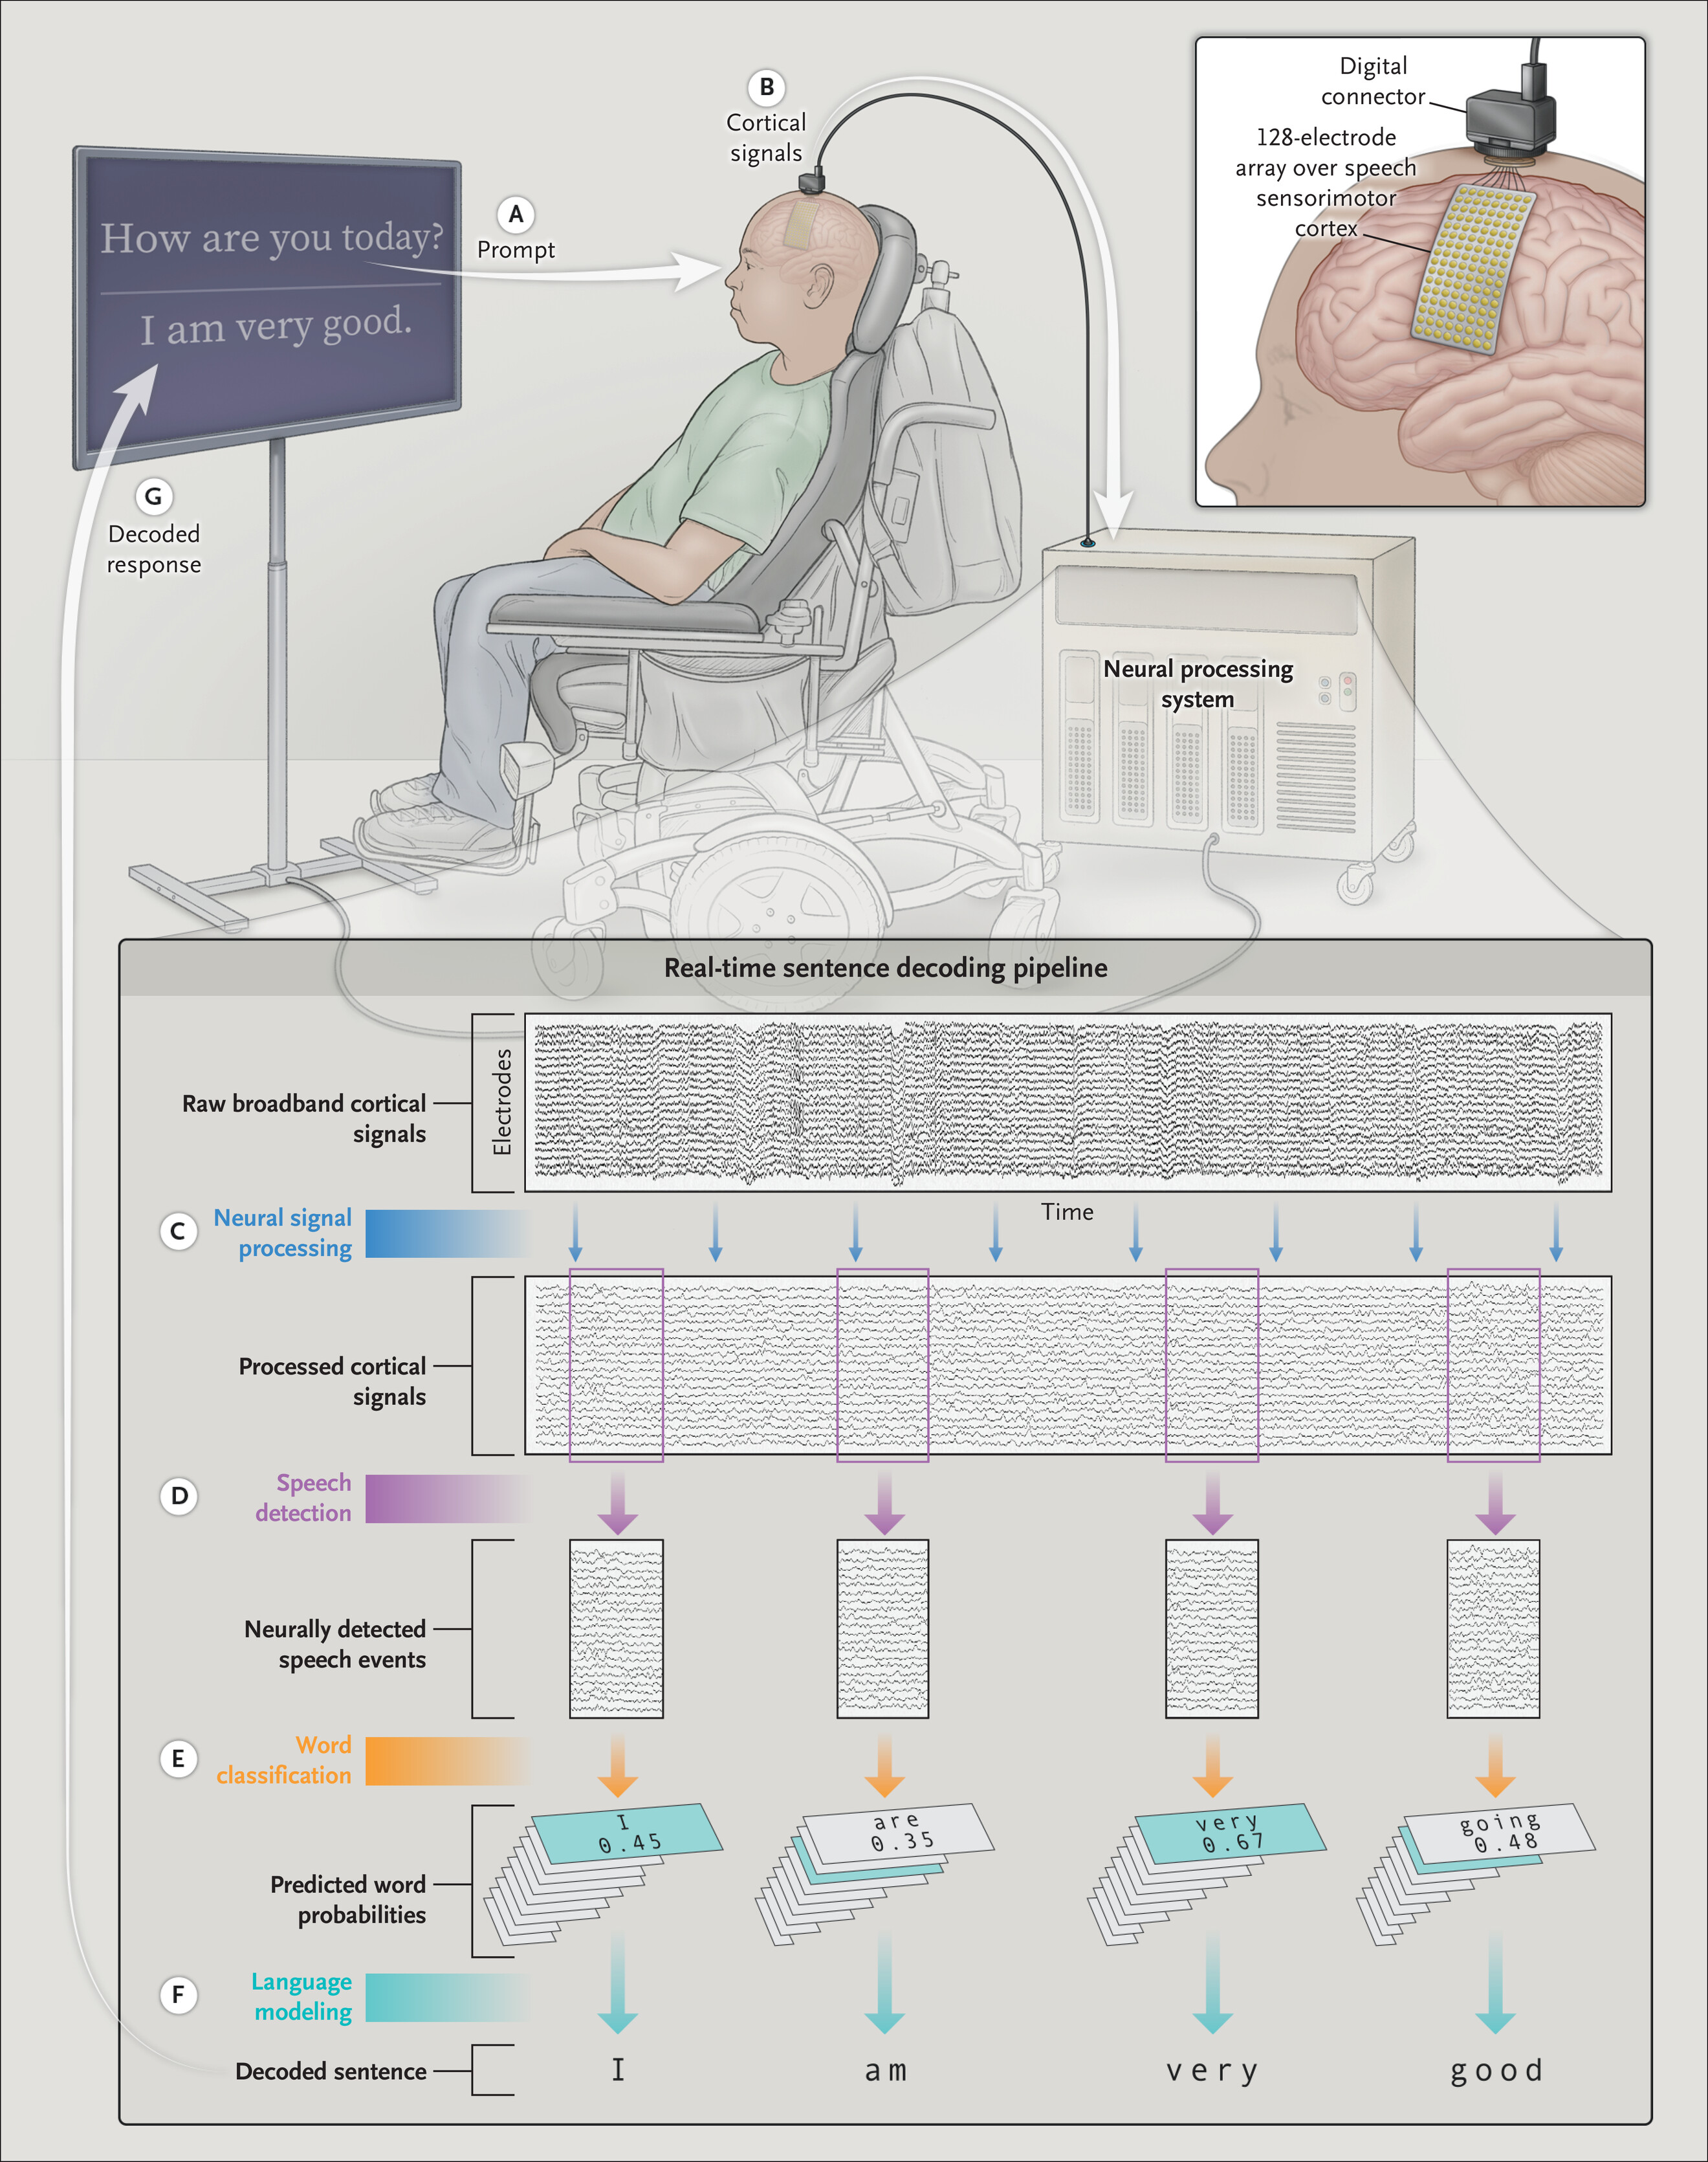
\includegraphics[height=0.6\textheight]{figures/Moses_2021_nejm.jpg} 

\tiny{Figure from Moses et al. (2021) NEJM.}
\end{center}
\end{column}
\end{columns}


\end{frame}


%%%%%%%%%%%%%%%%%%%%%%%%%%%%%%%%%%%%

\begin{frame}
\frametitle{History: Early work (1990s-2000s)}

\begin{columns}
\begin{column}{0.48\textwidth}
\textbf{Key milestones:}

\small
\begin{itemize}
\setlength\itemsep{0.3em}
\item 1999-2002: Nicolelis lab - monkeys controlled robotic arms

\item 2002: Donoghue lab - cursor control, foundation for BrainGate
\end{itemize}


\end{column}
\begin{column}{0.48\textwidth}
\begin{center}
% Figure: Monkey controlling robotic arm or cursor
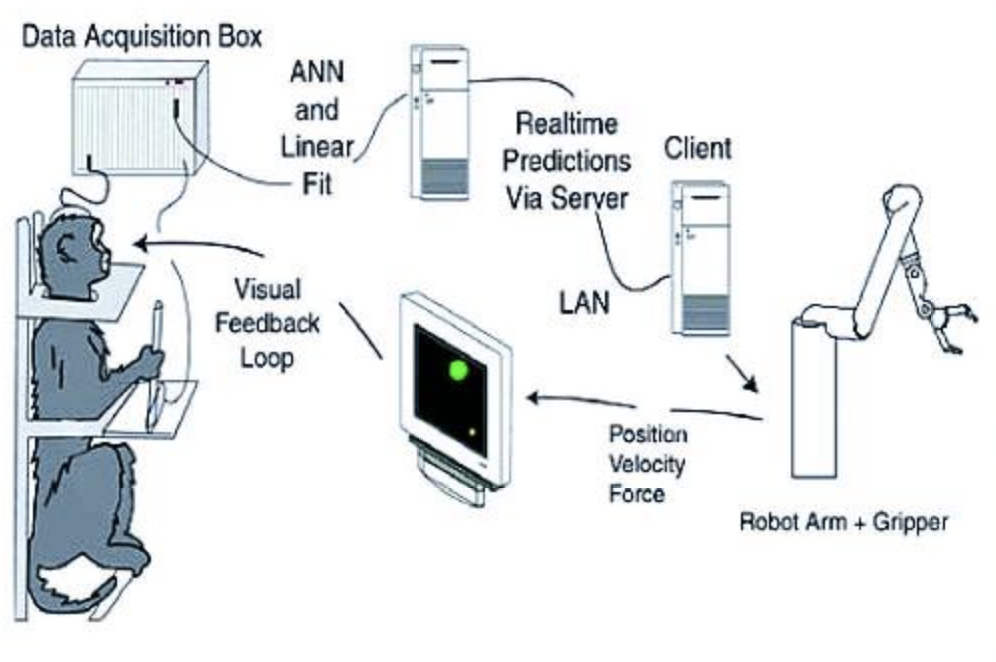
\includegraphics[width=\textwidth]{figures/Carmena_2003_PLOS.png}

\vspace{0.2cm}

\tiny{From Carmena et al. (2003) PLOS Biology}
\end{center}
\end{column}
\end{columns}

\end{frame}

%%%%%%%%%%%%%%%%%%%%%%%%%%%%%%%%%%%%

\begin{frame}
\frametitle{Modern BCIs: BrainGate system (2012)}

\begin{center}
% Figure: BrainGate electrode array and participant using robotic arm
% Source: Hochberg et al. (2012) Nature - shows participant T2 reaching with robotic arm
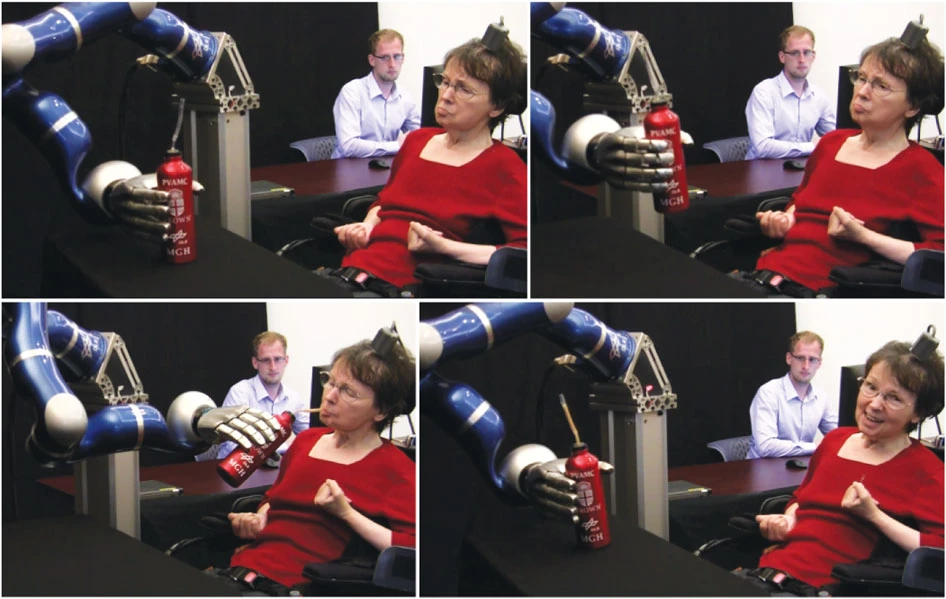
\includegraphics[width=0.9\textwidth]{figures/Hochberg_2012_braingate.png} 

\vspace{0.3cm}

\small{From Hochberg et al. (2012) Nature. Participant with tetraplegia using BrainGate system to control robotic arm and drink coffee independently.}
\end{center}

\end{frame}

%%%%%%%%%%%%%%%%%%%%%%%%%%%%%%%%%%%%

\begin{frame}
\frametitle{Modern BCIs: Speech restoration (2023)}

\begin{center}
% Figure: Chang lab speech BCI showing electrode placement and decoded speech
% Source: Moses et al. (2021) NEJM OR Metzger et al. (2023) Nature
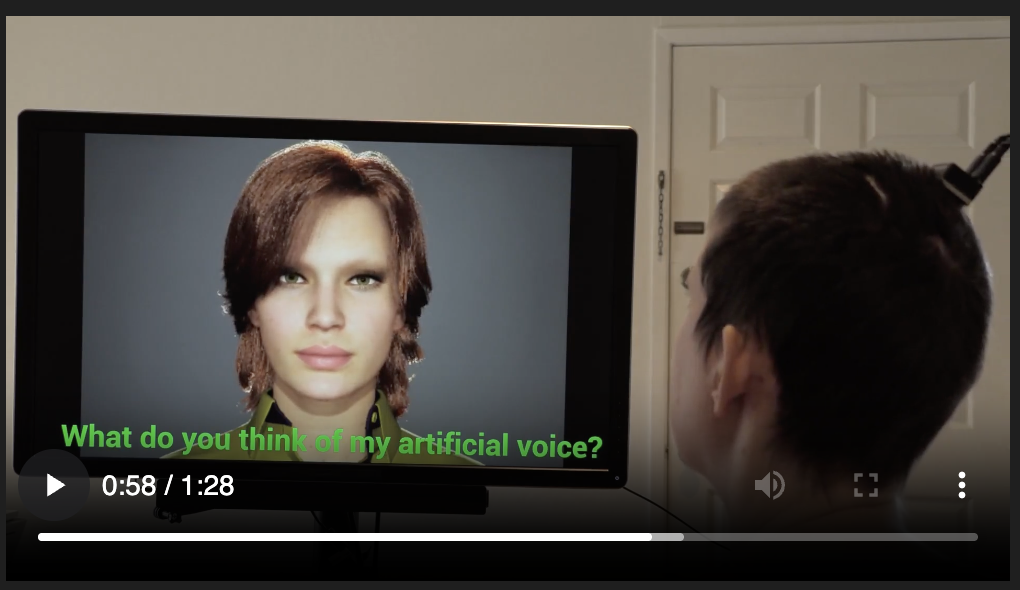
\includegraphics[width=0.9\textwidth]{figures/Metzger_2023_speech_bci.png}

\vspace{0.3cm}

\small{From Metzger et al. (2023) Nature. (See Video) Speech BCI decodes attempted speech from motor cortex, synthesizing speech and facial expressions at conversational speed.}
\end{center}

\end{frame}

%%%%%%%%%%%%%%%%%%%%%%%%%%%%%%%%%%%%

\begin{frame}
\frametitle{BCIs in industry: Moving beyond the lab}

% \begin{columns}
% \begin{column}{0.48\textwidth}
\textbf{Commercial development:}

\small
\begin{itemize}
\setlength\itemsep{0.3em}
\item \textbf{Neuralink} (Elon Musk)
\begin{itemize}
\scriptsize
\item High-density electrode arrays
\item 2024: First human implant
\end{itemize}

\item \textbf{Synchron}
\begin{itemize}
\scriptsize
\item Minimally invasive (via blood vessel)
\item FDA approval trials ongoing
\end{itemize}

\item \textbf{Paradromics, Blackrock Neurotech}
\begin{itemize}
\scriptsize
\item Clinical-stage systems
\item Focus on speech and movement
\end{itemize}
\end{itemize}

% \end{column}

% \begin{column}{0.48\textwidth}
% \begin{center}
% % Figure: Comparison of different BCI systems or industry timeline
% % Could use company logos, device photos, or Nature Reviews Neuroscience overview
% % \includegraphics[width=\textwidth]{bci_industry_systems.png} TODO

% \vspace{0.2cm}

% \tiny{Various commercial BCI systems in development}
% \end{center}
% \end{column}
% \end{columns}

\end{frame}

%%%%%%%%%%%%%%%%%%%%%%%%%%%%%%%%%%%%


%%%%%%%%%%%%%%%%%%%%%%%%%%%%%%%%%%%%

\begin{frame}
\frametitle{The decoding problem: A regression challenge}

\begin{columns}
\begin{column}{0.48\textwidth}
\textbf{Statistical framework}:

\small
\begin{equation*}
\text{Intended Action} = f(\text{Neural Activity})
\end{equation*}

\begin{itemize}
\setlength\itemsep{0.3em}
\item \textbf{Response}: Cursor position, word, arm movement

\item \textbf{Predictors}: Neural activity from 100s of electrodes

\item \textbf{Methods}: Linear regression, GLMs, machine learning
\end{itemize}
\end{column}

\begin{column}{0.48\textwidth}
\begin{center}
% Figure: Neural tuning curves or decoding performance
% Source: Pandarinath et al. (2017) eLife OR Gilja et al. (2012) Nature Neuroscience
% \includegraphics[width=\textwidth]{neural_decoding_performance.png} TODO

\vspace{0.2cm}

% \tiny{From Pandarinath et al. (2017) eLife}
\end{center}
\end{column}
\end{columns}

\end{frame}

%%%%%%%%%%%%%%%%%%%%%%%%%%%%%%%%%%%%

\section{Dataset: Neural Latents Benchmark}

\subsection{Data: Neural activity and cursor movement}

%%%%%%%%%%%%%%%%%%%%%%%%%%%%%%%%%%%%

\begin{frame}
\frametitle{Introducing the MC\_maze dataset}

\begin{columns}
\begin{column}{0.6\textwidth}
\textbf{What is \webLink{https://neurallatents.github.io/datasets\#mcmaze}{MC\_maze}?}

\begin{itemize}
\setlength\itemsep{0.4em}

\item A \textit{public, open-source} dataset from neuroscience research

\item Records from a monkey playing a computer game (reaching a cursor to targets)

\item Contains simultaneous measurements of:
\begin{itemize}
\item \textbf{Neural signals}: Firing rates from 100+ neurons in motor cortex
\item \textbf{Behavior}: Cursor position and velocity over time
\end{itemize}

\end{itemize}
\end{column}
\begin{column}{0.4\textwidth}
    \begin{center}
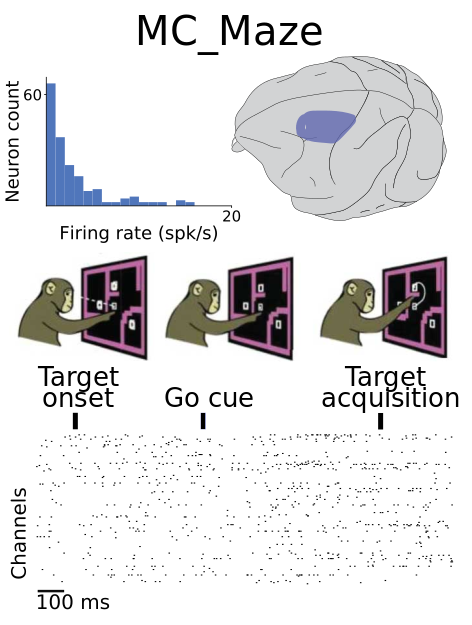
\includegraphics[width=\textwidth]{figures/maze_fig1.png}
    \end{center}
\end{column}
\end{columns}


\end{frame}

%%%%%%%%%%%%%%%%%%%%%%%%%%%%%%%%%%%%

\begin{frame}
\frametitle{The data structure: What does each observation represent?}

\textbf{Temporal data at millisecond resolution}

\vspace{0.3cm}

Each row = one \textit{time bin} (e.g., 50 milliseconds)

\vspace{0.3cm}

\begin{columns}
\begin{column}{0.48\textwidth}
\textbf{Predictors (Neural activity):}
\small
\begin{itemize}
\item Neuron 1 firing rate
\item Neuron 2 firing rate
\item ...
\item Neuron 100+ firing rate
\end{itemize}

\textit{Firing rate} = spikes per unit time
\end{column}

\begin{column}{0.48\textwidth}
\textbf{Response (Behavior):}
\small
\begin{itemize}
\item Cursor X position
\item Cursor Y position
\item Cursor X velocity
\item Cursor Y velocity
\end{itemize}

\textit{Velocity} = change in position over time
\end{column}
\end{columns}

\vspace{0.3cm}

\textbf{Goal}: Predict cursor position/velocity from neural firing rates

\end{frame}

%%%%%%%%%%%%%%%%%%%%%%%%%%%%%%%%%%%%

\begin{frame}
\frametitle{Motor cortex neurons encode movement intent}

\begin{center}
% Figure: Example neural tuning curve or raster plot
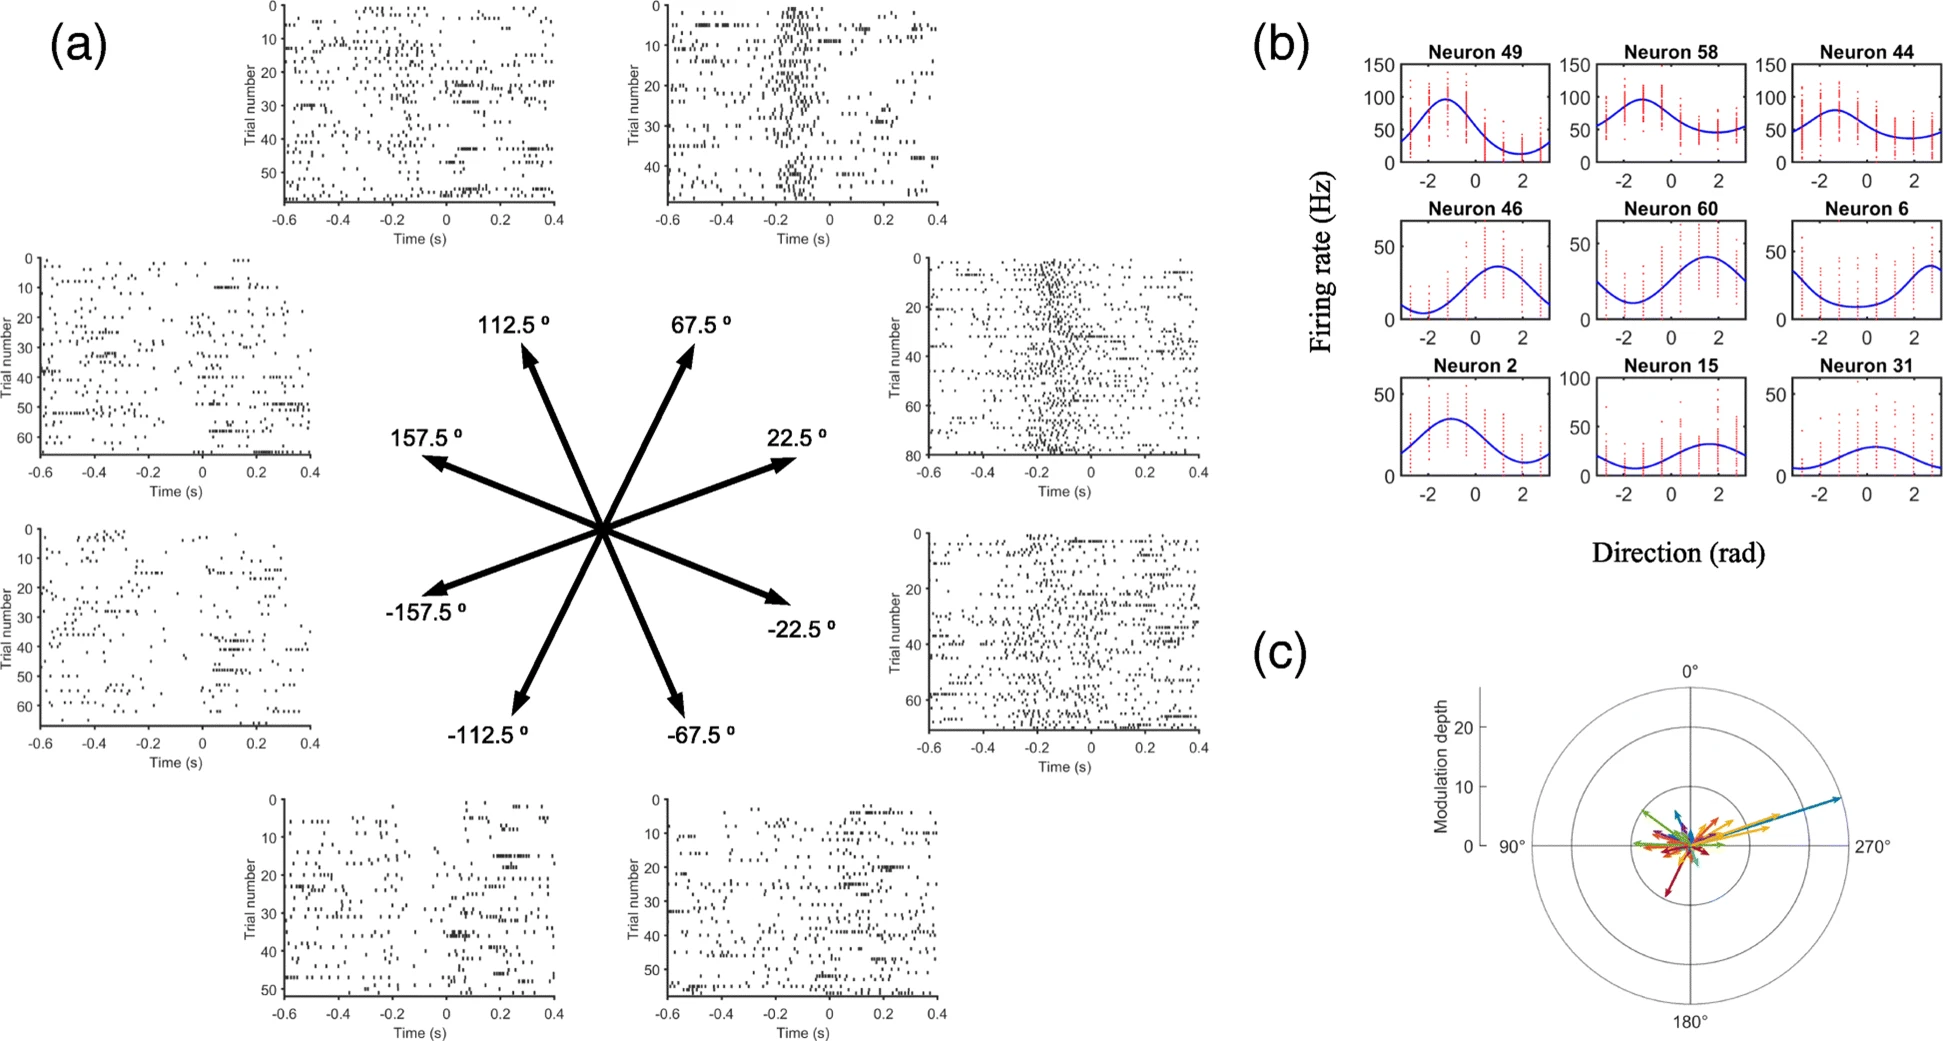
\includegraphics[width=0.8\textwidth]{figures/Tam_2019_BMC_Biomed_Eng.png}

\tiny{From Tam et al. (2019) BMC Biomed Eng}

\end{center}
\vspace{-0.4cm}

\begin{itemize}

\item (a) A neuron ``fires more'' when the monkey intends to move in its preferred direction

\item (b, c) Different neurons prefer different movement directions

\item By observing firing rates across many neurons, we can infer intended movement

\end{itemize}

\vspace{0.3cm}

\textbf{Statistical question}: How well can we predict cursor movement from firing rates?

\begin{itemize}
\item Linear regression: $\text{Position}_t = \beta_0 + \beta_1 \text{Neuron}_1(t) + \cdots + \beta_p \text{Neuron}_p(t) + \epsilon$
\end{itemize}

\end{frame}

%%%%%%%%%%%%%%%%%%%%%%%%%%%%%%%%%%%%

\begin{frame}
\frametitle{Challenges specific to this dataset}

\textbf{Why MC\_maze is realistic for BCIs:}

\begin{itemize}
\setlength\itemsep{0.4em}

\item \textbf{High dimensionality}: 100+ neural predictors vs. a few response variables

\item \textbf{Temporal correlation}: Consecutive time bins are not independent

\item \textbf{Neural noise}: Firing rates are variable and noisy

\end{itemize}

\end{frame}

%%%%%%%%%%%%%%%%%%%%%%%%%%%%%%%%%%%%

\section{R demonstration: Visualizing BCI data}

\subsection{If you're interested in this topic...}


%%%%%%%%%%%%%%%%%%%%%%%%%%%%%%%%%%%%
% End document
%%%%%%%%%%%%%%%%%%%%%%%%%%%%%%%%%%%%

\end{document}